\chapter{Theoretical framework}
\label{chap:chapter_2}
An introduction to the Standard Model is reported, as well as recent results about the Higgs boson and theoretical motivations for the study of its self-coupling.

\section{The Standard Model}

With Standard Model (SM), we group a set of theories that as of date explain the behaviour of matter at high energies, taking into account three of the four fundamental interactions. 

In the SM, the elementary particles are divided into two different categories: bosons, with integer spin, which follow the Bose-Einstein statistics, and are the mediators of the fundamental interactions, and fermions, with semi-integer spin, which follow the Fermi-Dirac statistics and compose matter.

We consider the following Lagrangian:

\begin{equation}
    \mathcal{L} = -\frac{1}{4}F_{\mu \nu}F^{\mu \nu} + i\bar{\psi}\slashed{D}\psi + \text{h.c.}
\end{equation}

where:
\begin{equation}
     -\frac{1}{4}F_{\mu \nu}F^{\mu \nu} = - \frac{1}{4}W_a^{\mu\nu} W_{\mu\nu}^a - \frac{1}{4} B^{\mu\nu}B_{\mu\nu} -\frac{1}{4}G_{\mu \nu}^a G^{\mu \nu}_a
\end{equation}

is the Yang-Mills part, which takes into account the interaction of the mediators among themselves, and:
\begin{align}
    &i\bar{\psi}\slashed{D}\psi = \bar{L}_i i\gamma^{\mu}(\partial_{\mu}\delta_{ij} + i g \frac{(\tau_a)_{ij}}{2}W_{\mu}^a + i g' \frac{Y_{ij}}{2}B_{\mu})L_j + \\ \bar{R}_i &i\gamma^{\mu}(\partial_{\mu}\delta_{ij} + i g' \frac{Y_{ij}}{2}B_{\mu})R_j 
    + \Bar{q}_i(i\gamma^{\mu}\partial_{\mu} \delta_{ij} - i g (T_a)_{ij}A^a_{\mu})q_j \nonumber
\end{align}
is the fermionic part.\\
In particular, we consider the Glashow-Weinberg-Salam theory for describing the electroweak interactions and the Quantum Chromodynamics (QCD) for describing the strong interaction.\\
Both QCD and the electroweak theory are gauge theories. \\
Briefly, a gauge theory is a theory where the symmetry described by the symmetry group is not only global, but also local. This means we can perform local transformations on the field while keeping the whole Lagrangian invariant, as long as a transformation on the potential field is performed as well.\\



For this reason, if we perform a transformation of the form:
\begin{equation}
    \phi \rightarrow \phi e^{i\theta(x)}
\end{equation}
on the field, we also have to perform a transformation of the form:
\begin{equation}
    A_{\mu} \rightarrow A_{\mu} -\frac{1}{\alpha}\partial_{\mu}\theta, 
\end{equation}
on the potential field, where $\alpha$ is the coupling constant of the interaction field.\\


\subsection{Electroweak interactions}

The Glashow-Weinberg-Salam theory for the electroweak interaction has the following Lagrangian:

\begin{equation}
    \mathcal{L} = - \frac{1}{4}W_a^{\mu\nu} W_{\mu\nu}^a - \frac{1}{4} B^{\mu\nu}B_{\mu\nu} + \bar{L} i\gamma^{\mu}(\partial_{\mu} + i g \frac{\tau_a}{2}W_{a\mu} + i g' \frac{Y}{2}B_{\mu})L +
    \label{ew_eq}
\end{equation}
\begin{equation*}
    \bar{R} i\gamma^{\mu}(\partial_{\mu} + i g' \frac{Y}{2}B_{\mu})R,
\end{equation*}

where:
\begin{equation}
    L = \begin{pmatrix}
        \nu \\ l
    \end{pmatrix}_L \hspace{20pt} R = l_R,
\end{equation}
$W_{\mu\nu}$ is the field for the bosons of the weak interaction with generators $\tau_a$ from the group $SU(2)_L$, $B_{\mu\nu}$ is the field for the electromagnetic interaction with generator $\frac{Y}{2}$ from the group $U(1)$.

So it predicts the existence of a doublet of fermions, the leptons $\nu \text{ and } l $, and four bosons (3 from  $SU(2)$ and 1 from $U(1)$).
These particles have two quantum numbers, the weak isospin associated with $SU(2)$ and the hypercharge associated with $U(1)$.

The electroweak theory is chiral, meaning that particles with different chiralities (left or right) will act differently under electroweak interactions. 
In particular, only left particles will interact weakly with coupling $g$, while the electromagnetic part acts similarly on both chiralities with coupling $g'$.

This also means that electroweak interactions can't have a mass term because a term of the form $L * R$ would break the symmetry of the global group $SU(2)_L x U(1)$, not being a scalar in the chirality.

\subsection{Quantum Chromodynamics}

Quantum Chromodynamics (QCD) has the following Lagrangian:

\begin{equation}
    \mathcal{L} = -\frac{1}{4}F_{\mu \nu}F^{\mu \nu} + \bar{\psi}(i\slashed{D} - m)\psi %va fixata
\end{equation}
where $\psi$ are three-component vectors in the colour quantum number.


It has a gauge symmetry SU(3) of colour and hypothesizes the existence of a fundamental fermion called quark, and a gauge boson called gluon.
These particles carry a quantum number called colour. Only coloured particles can interact strongly.

Quarks also carry hypercharge and weak isospin, so they also interact electromagnetically and weakly. In particular, we can define two species of quarks, up and down, based on the sign of their electrical charge.\\

In the perturbative approach to the theory, we can write the $\beta$-function, which describes the dependence of the coupling constant $g$ to the energy scale $\mu$:
\begin{equation}
    g^2 = \dfrac{1}{\beta_0 \ln\left(\frac{\mu^2}{\Lambda_{QCD}}\right)}, \beta_0 > 0
\end{equation}
We can observe that, because of the sign of $\beta_0$, the coupling constant goes to 0 at higher energies, and, on the other hand, it diverges for low energies. This latter behaviour is what is called \emph{confinement}, and it is one of the characteristic aspects of QCD.\\

Confinement implies that there can't be asymptotic states with color.

\subsection{Mass terms in the SM}
A mass term for the SM must be a scalar under the whole group $SU(3)x SU(2)_Lx U(1)_Y$.


QCD is not a chiral theory, so it acts the same on particles with left and right chirality. 
If we consider the fermionic term of the QCD Lagrangian, and explicitly write it for fields with defined chirality, we find:

\begin{equation}
    \bar{\psi} (i\partial_{\mu}\gamma^{\mu}  - m ) \psi =  (\bar{\psi}_L + \bar{\psi}_R) (i\partial_{\mu}\gamma^{\mu}  - m ) (\psi_L + \psi_R) =
\end{equation}
\begin{equation*}
    = \bar{\psi}_L\partial\psi_L + \bar{\psi}_R\partial\psi_R - m\bar{\psi}_L\psi_R - m\bar{\psi}_R\psi_L
\end{equation*}

where:
\begin{equation*}
    \psi_L = P_L \psi = \frac{1}{2}(1- \gamma_5)\psi, \hspace{20pt} \psi_R = P_R\psi = \frac{1}{2}(1+ \gamma_5)\psi
\end{equation*}
and terms cancel out due to the orthogonality of projectors $P_L$ and $P_R$ and the properties of $\gamma$ matrices.

We can observe that the term $ - m(\bar{\psi}_L\psi_R + \bar{\psi}_R\psi_L)$ is a scalar under chirality.

This means that, if the whole Lagrangian is invariant under chirality, a term of mass for particles with defined chirality can exist.

However, when considering both theories at the same time, that is not the case anymore. In fact, when taking into account the whole group $SU(3)xSU(2)_LxU(1)_Y$ this is not chiral invariant anymore due to the chirality of $SU(2)_L$. 

So, the Standard Model defined like this doesn't take into account the mass of elementary particles, which are instead observed experimentally.

Another experimental proof that the SM can't explain is the existence of multiple types (flavours) of quarks and multiple doublets of leptons.

To solve both of these problems, the ideas of spontaneous symmetry breaking and the Higgs model were introduced.

\section{Introduction to symmetry breaking}

Symmetry breaking is a process that happens when some kind of symmetry of the physical theory is lost.

In physics, three kinds of symmetry breaking are defined:

\begin{itemize}
    \item \textbf{Explicit symmetry breaking}: the Lagrangian of the system has a term that explicitly breaks the symmetry;
    \item \textbf{Spontaneous symmetry breaking}: the Lagrangian is overall symmetric, so the equations of motions are symmetric, but lowest-energy vacuum solutions are not symmetric;
    \item \textbf{Anomalous symmetry breaking}: there's an additional term in the action of the system that makes the equation of motion non-symmetric.
\end{itemize}

The symmetry break that gives the Higgs field is of the second type.

\subsection{Abelian case: real field}
Let us consider the following Lagrangian:
\begin{equation}
    \mathcal{L} = \frac{1}{2} (\partial_{\mu}\phi)(\partial^{\mu}\phi) - V(\phi),  \quad V(\phi) = \frac{1}{2}\mu^2\phi^2 + \frac{1}{4}\lambda\phi^4
\end{equation}
for a scalar field $\phi$. \\


The quartic potential is the simplest potential that can bring out the symmetry breaking.\\
There are two possible cases:
\begin{itemize}
    \item $\mu^2>0$: the vacuum minimum is unique, $\phi = 0$;
    \item $\mu^2<0$: the vacuum solutions for $V(\phi)$ are non-degenerate, and they are:
\begin{equation}
   \langle\phi\rangle \equiv v = \pm \sqrt{\frac{\mu^2}{\lambda}}, \quad v \in \mathbb{R} \label{v_relation}
\end{equation}
\end{itemize}

We can redefine the potential as:
\begin{equation}
    V(\phi) = \frac{1}{4}\lambda(\phi^2- v^2)^2
\end{equation}
and by considering a new field $\Tilde{\phi} \equiv \phi - v$ that describes the fluctuations of the field around the minimum we obtain a new Lagrangian:
\begin{equation}
    \mathcal{L} = \frac{1}{2} (\partial_{\mu}\Tilde{\phi})(\partial^{\mu}\Tilde{\phi}) +\lambda v^2\Tilde{\phi}^2 - \lambda v \Tilde{\phi}^3 - \frac{1}{4}\lambda\phi^4
\end{equation}
We can identify a mass term multiplying the quadratic field:
\begin{equation}
    m = \sqrt{-2 \mu^2}
\end{equation}
\subsection{Abelian case: complex field}
In this case, we consider the following Lagrangian:
\begin{equation}
    \mathcal{L} = \frac{1}{2} (\partial_{\mu}\phi^\dagger)(\partial^{\mu}\phi) - \mu^2\phi^\dagger\phi - \lambda (\phi^\dagger\phi)^2
\end{equation}

This Lagrangian has global symmetry $U(1)$, that is, it is invariant under the transformations:
    

\begin{equation}
\begin{cases}
    \phi \rightarrow e^{-i \alpha}\phi \\
    \phi^{\dagger} \rightarrow e^{i \alpha} \phi^{\dagger}
\end{cases}
\end{equation}
In this case, as well, we can distinguish two cases:
\begin{itemize}
    \item $\mu^2> 0$: unique solution in 0;
    \item $\mu^2<0$: there are infinite sets of solutions, as can be seen from the fig \ref{higgs}.
\end{itemize}
\begin{figure}
    \centering
    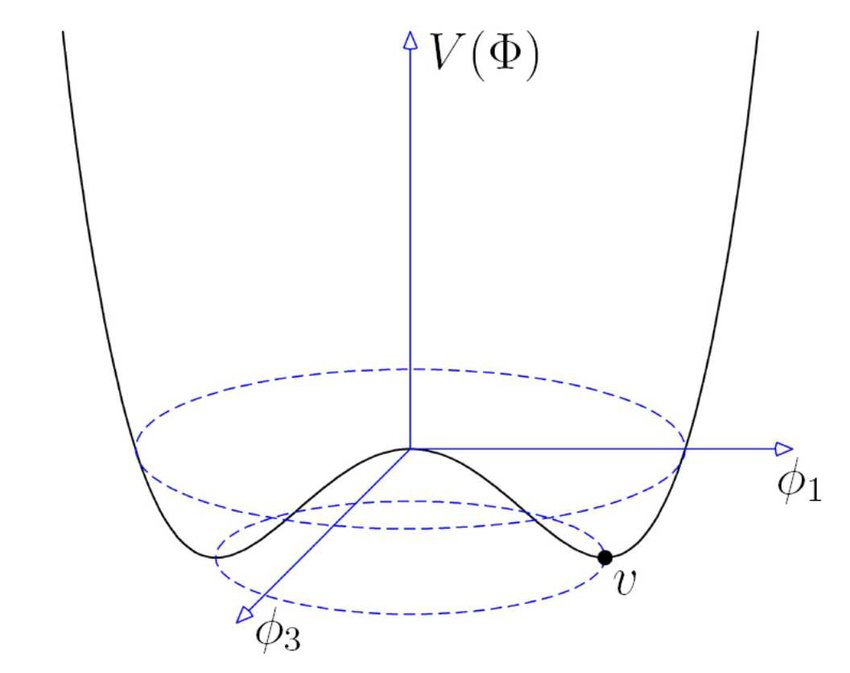
\includegraphics[width=\textwidth]{images/higgs_potential.jpg}
    \caption{Higgs potential, and its typical form. A vacuum solution is highlighted}
    \label{higgs}
\end{figure}
We define the complex components of the fields as follows:
\begin{equation}
    \phi = \phi_1 + i \phi_2
\end{equation}
and we choose the following minimum:
\begin{equation}
    \begin{cases}
        \langle\phi_1\rangle_0 \equiv v = \sqrt{-\dfrac{\mu^2}{\lambda}} \\
        \langle \phi_2\rangle_0 = 0
    \end{cases}
\end{equation}

We define two new fields around the value of the minimum:
\begin{equation}
    \begin{cases}
        \eta = \phi_1 - v\\
        \chi = \phi_2
    \end{cases}
\end{equation}
Substituting the new fields in the Lagrangian we obtain:
\begin{equation}
    \mathcal{L} = \frac{1}{2}(\partial_{\mu}\eta)(\partial^{\mu\eta} + \frac{1}{2}(\partial_{\mu}\chi)(\partial^{\mu}\chi) +\mu^2 \eta^2 
\end{equation}
\begin{equation*}
    - \lambda\left[\frac{1}{4}\left(\eta^2 +\chi^2\right)^2 + v \eta \left(\eta^2 + \chi^2\right)\right] +\text{const.}
\end{equation*}
We can observe that now we obtain two particles, $\eta$ and $\chi$.\\
In particular, $\eta$ is a massive particle with mass:
\begin{equation*}
    m_{\eta} = \sqrt{-2\mu^2}
\end{equation*}
while $\chi$ is massless.\\

We can see that this case is of our interest because it resembles the physical case of the electroweak interaction (a massive particle and a massless one).
However, the complex scalar field theorizes only two particles, while from the experiments we know there are four bosons for this interaction: W$^{\pm}$, Z and the photon.\\This means we have to find a bigger group that can give us 4 bosons. \\
In particular, we need 4 gauge bosons. A specific discussion of spontaneous symmetry breaking in the presence of a gauge symmetry is discussed in the appendix.

\subsection{Non-Abelian case and the Higgs mechanism}
The Higgs mechanism was proposed in 1964 separately by P. Higgs \cite{higgs_art} and R. Brout and F. Englert \cite{brout_art}.\\
We consider the gauge group $SU(2)xU(1)$ \cite{weinberg} and we perform a symmetry break on the global group with the pattern:
\begin{equation}
    SU(2)_L x U(1)_Y \rightarrow U(1)
\end{equation}
We choose to leave a remaining global $U(1)$ symmetry to describe the photon, which stays massless.\\
We take the electroweak Lagrangian from equation \ref{ew_eq}, and we add an additional field, $\Phi$:
\begin{equation}
    \Phi =
    \begin{pmatrix}
        \phi^+\\ \phi_0
    \end{pmatrix}
\end{equation}
This field is what parametrizes the Higgs mechanism. $\phi^+$ is charged while $\phi_0$ is neutral.\\
The complete Lagrangian is:
\begin{equation}
    \mathcal{L}= -\frac{1}{4}A_{\mu\nu}A^{\mu\nu} -\frac{1}{4}B_{\mu\nu}B^{\mu\nu} + \left(D_{\mu}\Phi\right)^{\dagger}\left(D^{\mu}\Phi\right) - V(\Phi^{\dagger}\Phi), 
\end{equation}
where:
\begin{equation}
   \mathcal{L} =  -\frac{1}{4}A_{\mu\nu}A^{\mu\nu}
\end{equation}
is the Yang-Mills Lagrangian for the $SU(2)$ bit, while:
\begin{equation}
    \mathcal{L} = -\frac{1}{4}B_{\mu\nu}B^{\mu\nu}
\end{equation}
takes into account the $U(1)$ part, and:
\begin{equation*}
    V(\Phi^{\dagger}\Phi) = \mu^2(\Phi^{\dagger}\Phi) + \lambda(\Phi^{\dagger}\Phi)^2
\end{equation*}
is the usual quartic potential for the $\Phi$ field, the Higgs field.

We consider $\mu^2<0$ and choose the minimum value of the field to be:
\begin{equation}
    \Phi_{min} = \frac{1}{\sqrt{2}}\begin{pmatrix}
        0 \\ v
    \end{pmatrix}, \quad v \in \mathbb{R}
\end{equation}
As we've already done before, we can parameterize the fluctuations around $\phi_{min}$, and by fixing the gauge as well we find:
\begin{equation}
    \Phi(x) =\frac{1}{\sqrt{2}} \begin{pmatrix}
        0 \\ v + \rho(x)
    \end{pmatrix}
\end{equation}
where $1/\sqrt{2}$ is a conventional normalization.\\

Substituting in the Lagrangian, we can find:
\begin{equation}
    \mathcal{L} = - \frac{1}{4} A_{\mu\nu}A^{\mu\nu} -\frac{1}{4} B_{\mu\nu}B^{\mu\nu} + \frac{1}{2}\partial_{\mu}\rho\partial^{\mu}\rho -V\left(\frac{(v + \rho)^2}{2}\right) +
\end{equation}
\begin{equation*}
    \frac{(v+ \rho)^2}{8}\left[\left(g' B_{\mu} - gA_{\mu}^{(3)}\right) \left(g' B^{\mu} - g A^{(3)\mu}\right) +g^2\left(A_{\mu}^{(1)} A^{(1)\mu} + A_{\mu}^{(2)} A^{(2)\mu}  \right) \right]
\end{equation*}
We can see that we can consider a linear combination of $B_{\mu}$ and the neutral element of the multiplet $A_{\mu}$.\\
That is, we can define new fields:
\begin{equation}
    W_{\mu}^{\pm}= \frac{1}{\sqrt{2}}\left(A_{\mu}^{(1)}\mp A_{\mu}^{(2)}\right), \quad m_W = \frac{vg}{2}
\end{equation}
\begin{equation}
    Z_{\mu} = \frac{1}{\sqrt{g^2 + g'^2}}\left( - g A_{\mu} ^{(3)} + g' B_{\mu} \right), \quad m_Z = \frac{v}{2}\sqrt{g^2 + g'^2}
\end{equation}
\begin{equation}
    A_{\mu} = \frac{1}{\sqrt{g^2 + g'^2}}\left(g A_{\mu} ^{(3)} + g' B_{\mu} \right), \quad m_A = 0
\end{equation}
Requesting the known form for $v$ we can also find the mass of the Higgs boson: $m_H = \sqrt{-2\mu^2}$, as expected from the previous sections, that however depends on a free parameter of the theory, $\mu$.\\
As a side note, we can notice that in this way the mass term for the three fields becomes:
\begin{equation}
    \mathcal{L}_m = \frac{v^2}{4}\left[\left(\frac{g^2 + g'^2}{2}\right)Z_{\mu}Z^{\mu} + g^2 W_{\mu}^{\dagger}W^{\mu}\right]
\end{equation}
So, because of relation \ref{v_relation} the mass term is also proportional to $m_H^2$.
    

\subsection{Fermionic mass terms}

So far, we've seen how the Higgs mechanism allows the gauge boson to have mass (except for the photon, which is massless as expected).\\
We now briefly discuss the mass term for the fermionic side.\\
We define a mass term, called Yukawa interaction, with the form:
\begin{equation}
    \mathcal{L}_m = - G \Phi \Bar{\psi}_R \psi_L,
\end{equation}
where the presence of the doublet of the Higgs field allows the product between the left doublet and the right singlet, and $G$ is an arbitrary constant for each fermion.\\
This is sufficient to describe the leptonic sector, where the Higgs doublet selects only the charged lepton from the doublet (the Higgs mechanism doesn't take into account the mass of neutrinos), but it's not enough for the quarks.\\
Let's consider the mass term separately for up and down quarks:
\begin{equation}
    \mathcal{L}_m = -\left(\Bar{D}_L \Tilde{M}_D D_R + \Bar{U}_L \Tilde{M}_U U_R + \text{h.c.} \right), \quad \Tilde{M}= \frac{v}{\sqrt{2}}Y,
\end{equation}
where we are summing over the three families experimentally observed.\\
The two mass matrices, however, are not diagonal in this form. If we try to diagonalise them simultaneously to obtain the mass eigenstates, we find that it is impossible.\\
We can do it by rotating separately each field, and considering the overall matrix, now diagonal for both the left and right sectors:
\begin{equation}
    \begin{cases}
        U_L \rightarrow V_L^{(U)} U_L\\
        U_R \rightarrow V_R^{(U)} U_R
    \end{cases}
    \hspace{8pt} \Longrightarrow \hspace{8pt}M \equiv V_L^{(U)\dagger}\Tilde{M}V_R^{(U)} \hspace{12pt} \text{diagonal}
\end{equation}
and applying the same procedure on the down sector.\\
However, the newly defined fields introduce a new term in the charged current of the weak interaction:
\begin{equation}
    \mathcal{L}_{CC} = - \frac{g}{\sqrt{2}}\Bar{U}_L\gamma^{\mu}V_L^{(U)\dagger}V_L^{(D)}D_L + h.c. \equiv - \frac{g}{\sqrt{2}}\Bar{U}_L\gamma^{\mu}V_{CKM}D_L + h.c.
\end{equation}
The $V_{CKM}$ describes the mixing between up and down flavours, and introduces the CP violation in the weak sector. It is described by four independent parameters, 3 angles and a phase.\\

We can now write the complete Lagrangian for the SM:
\begin{equation}
    \mathcal{L} = -\frac{1}{4}F_{\mu\nu}F^{\mu\nu} + i\bar{\psi}\slashed{D}\psi +\text{h.c.} + \psi_i Y_{ij}\psi_j \Phi  +\text{h.c.} + |D_{\mu}\Phi|^2 -V(\Phi)
\end{equation}
We also report the characteristics of the SM particles in appendix \ref{app_particles}.

\section{Physics of the Higgs boson and recent results}
The Higgs boson was experimentally observed in 2012 at LHC simultaneously by the experiments CMS and ATLAS.\\
The most precise measurement of its mass by the CMS experiment \cite{art_nature_cms} is:
\begin{equation}
    m_H = 125.38 \pm 0.14 \text{GeV} 
\end{equation}
It is a scalar boson that has non-zero coupling with all fermions and with the weak bosons.
This means that there are multiple production modes, and multiple decay channels.\\
The magnitude of the coupling is deeply related to the particle's mass because, as we pointed out in the previous paragraphs, the coupling of the Higgs boson goes with $m_H^2$ for gauge bosons, and $m_H$ for fermions.
\subsection{Production modes}
The most common production modes in a hadronic accelerator as LHC  are the following: gluon-gluon fusion (ggH), vector boson fusion (VBF), vector-boson associated production (VH) and top pair associated production (ttH).\\
More in detail:
\begin{itemize}
    \item gluon-gluon fusion (ggF) is the predominant production mode, which accounts for approximately 85\% of the total cross-section. The interaction of the gluons with the Higgs boson is performed via quantum loops, as illustrated in fig. \ref{ggf_feynman}, where the predominant contribution is given by diagrams where the loop is made of top and, in lesser measure, bottom quarks;
    \item vector-boson fusion (VBF) is the second mode of production for relevance after ggH, and accounts for approximately 7\% of the total cross-section. The leading diagram, illustrated in fig.,  has two quarks, coming from the proton scattering, interact in the t or u channel, exchanging two vector bosons, which then interact as well through the s channel, emitting a Higgs boson. Because of the low transverse momentum exchange in comparison to the center of mass energy of the two interacting quarks, the signature of this mode of production is the presence of two jets with high rapidity. Furthermore, because this mode doesn't have diagrams that involve QCD, it has higher sensitivity in comparison to ggH;
    \item vector-boson associated production (VH) has an even lower production rate, accounting for 4\% of the total cross-section, and its main diagram has the radiation of a Higgs boson from a vector boson, as illustrated in fig. The signature of this mode is the presence of additional leptons (specifically $e$ and $\mu$) in the leptonic decay of the vector bosons involved;
    \item top pair associated production (ttH) is the mode with the least production rate among the ones listed, with a contribution of about 1\% over the total cross-section. However, it's interesting because its signature is consistent, having two quark top, which almost exclusively decay in Wb, and the decay products of these particles.
\end{itemize}


\begin{figure}[h]
    \centering
    \begin{subfigure}{0.55\textwidth}
    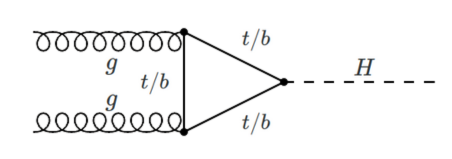
\includegraphics[width=\textwidth]{images/ggh.png}
    \caption{ggH production mode}
    \label{ggf_feynman}
    \end{subfigure}
    \hfill
    \begin{subfigure}{0.3\textwidth}
    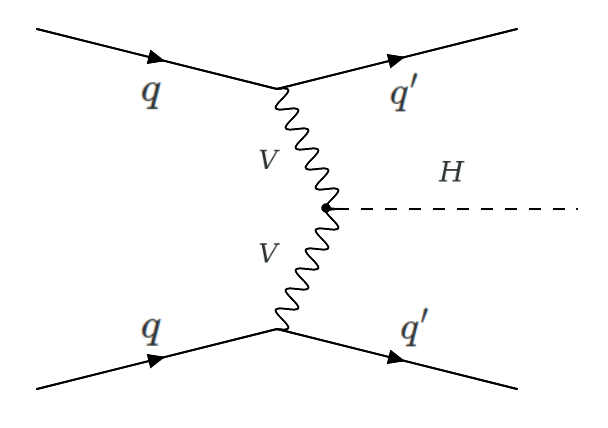
\includegraphics[width=\textwidth]{images/vbf.png}
    \caption{VBF production mode}
    \label{vbf_feynman}
    \end{subfigure}\vspace{5pt}
    \begin{subfigure}{0.55\textwidth}
    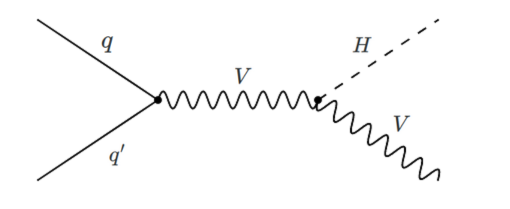
\includegraphics[width=\textwidth]{images/vh.png}
    \caption{VH production mode}
    \label{vh_feynman}
    \end{subfigure}\hfill
    \begin{subfigure}{0.3\textwidth}
    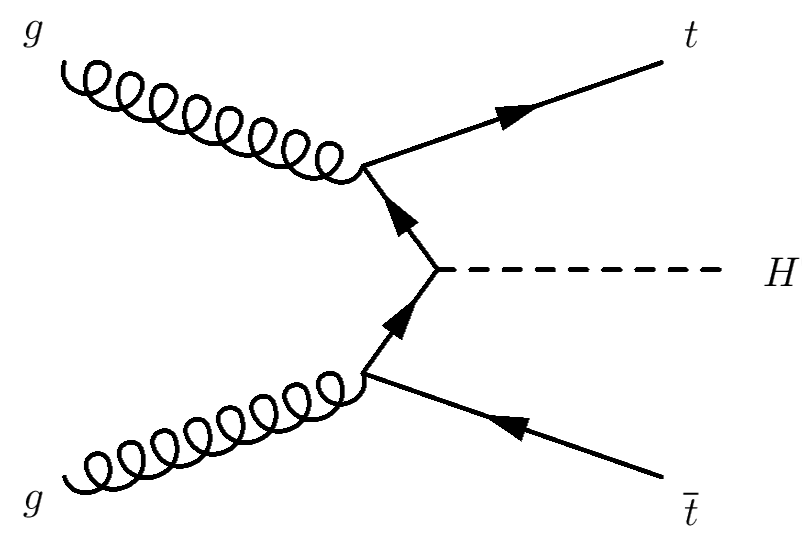
\includegraphics[width=\textwidth]{images/tth.png}
    \caption{ttH production mode}
    \label{tth_feynman}
    \end{subfigure}

    \caption{Feynman diagrams for leading production modes}
    \label{prod_feynman}
\end{figure}
A comprehensive plot of the theoretical cross-sections is presented in fig \ref{cross-section}, along with the pair production cross-section.

\begin{figure}
    \centering
    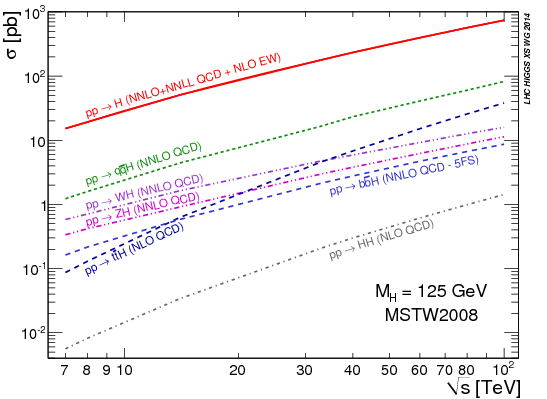
\includegraphics[width= \textwidth]{images/cross_section.png}
    \caption{Plot for the cross-sections as a function of CM energy}
    \label{cross-section}
\end{figure}
Table reports the theoretical cross-section divided by mode.
\begin{table}[ht]
    \centering
    \begin{tabular}{c|c}
         Process & Cross-section [pb]\footnotemark \\\hline
         ggF &  $48.6^{+2.7}_{-3.6}$ \\\hline
         VBF  & $3.78 \pm 0.08$\\\hline
         WH & $1.67\pm 0.03$\\\hline
         ZH & $0.88^{+0.04}_{-0.03}$ \\\hline
         t$\Bar{\text{t}}$H & $0.50^{+0.03}_{-0.04}$\\\hline 
    \end{tabular}
    \caption{Theoretical cross-sections for the predominant production modes for a Higgs boson of m$_H$ = 125 GeV and $\sqrt{s}$ = 13 TeV}
    \label{tab:cross-section}
\end{table}
\footnotetext{the unit of measure for cross-sections is the barn, which corresponds to $10^{-24} \text{cm}^2$. Usually, cross-section are in the order of pb ($10^{-12}$b) or fb ($10^{-15}$b)}
\subsection{Decay channels}
Because the Higgs boson is an unstable particle, it decays.\\
Its SM theoretical width is \cite{higgs_width}:
\begin{equation}
    \Gamma_H = 4.14 \pm 0.02 MeV \Longrightarrow \tau_H = \frac{\hbar}{\Gamma_H} \approx 1.6 \cdot 10^{-22} s
\end{equation}
Because of the small lifetime, the only way to detect the Higgs boson is through is decay products.\\ 
As already stated, the coupling of the Higgs boson is proportional to the mass of the particles (or the squared mass in the case of boson vectors), so the favoured channels are the ones with the gauge bosons and the third generation of fermions, that is, b quark and tau lepton, because the top quark is too heavy.\\
A comprehensive plot of the decay channels is presented in fig. \ref{higgs_br}, while table \ref{BR_teor} contains the theoretical branching ratios for the principal decay channels.\\
\begin{figure}[ht]
    \centering
    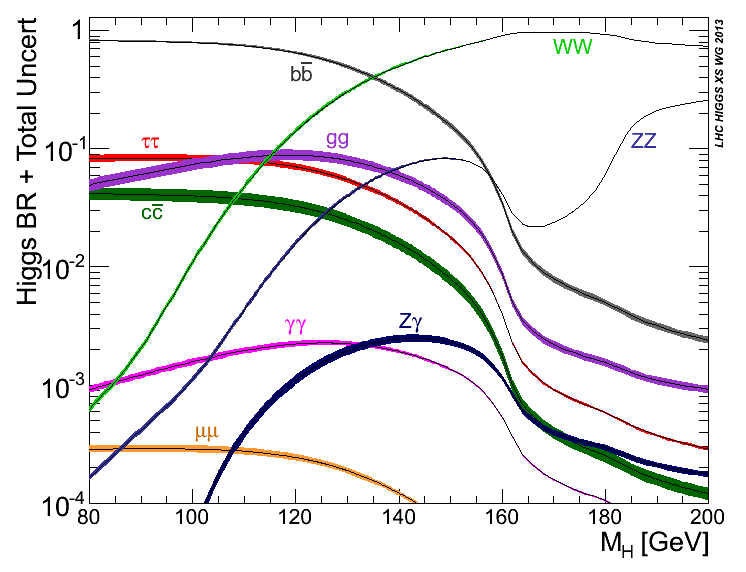
\includegraphics[width = \textwidth]{images/br.png}
    \caption{Branching ratios of the Higgs boson decay as a function of the mass}
    \label{higgs_br}
\end{figure}
\begin{table}[ht]
    \centering
    \begin{tabular}{c|c}
        Decay channel & Branching ratio [\%] \\\hline
        H $\rightarrow b\Bar{b} $ & 58.2\\  \hline
        H $\rightarrow$ $W^+ W^-$ & 21.4 \\\hline
        H $\rightarrow \tau^+ \tau^-$ & 6.27 \\\hline 
        H $\rightarrow$ ZZ & 2.6 \\\hline
        H $\rightarrow$ $\gamma\gamma$ & 0.22 \\\hline
        H $\rightarrow$ ZZ $\rightarrow$ $\mu, e$ & 0.03 \\\hline

    \end{tabular}
    \caption{Theoretical values for the branching fractions of the Higgs decay. The channel where the two Z from the Higgs decay go into charged leptons is called "\textit{golden channel}", because it provides a very high sensitivity}
    \label{BR_teor}
\end{table}
It should be noted that because the Higgs doesn't directly interact with the photon, the branching ratio $H\rightarrow\gamma\gamma$ provides us further information about the coupling of the particle inside the loop, which in this case can be either bosonic or fermionic, as it can be seen from fig. \ref{gamma_coupling}
\begin{figure}[ht]
    \centering
    \begin{subfigure}{0.4\textwidth}
        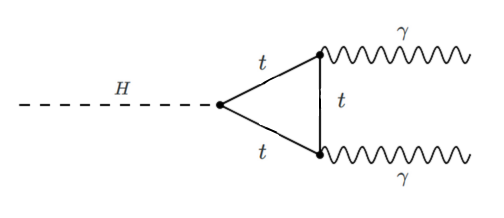
\includegraphics[width=\textwidth]{images/gamma_top.png}
        \caption{Fermionic loop}
        \label{gamma_top}
        \end{subfigure}
    \begin{subfigure}{0.4\textwidth}
        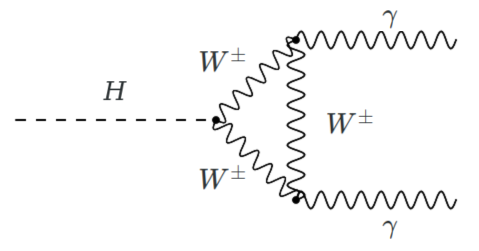
\includegraphics[width=\textwidth]{images/gammaW.png}
        \caption{Bosonic loop}
        \label{gamma_W}
        \end{subfigure}
    \caption{Feynman diagrams for the quantum loops that give the coupling of the Higgs boson with $\gamma$. In \ref{gamma_top} only the main contribution for the top is shown, while for \ref{gamma_W}, electrically charged bosons are the only boson admitted because of the coupling with the photon}
    \label{gamma_coupling}
\end{figure}
\subsection{Known issues}
Despite solving the mass problem for both the fermionic and bosonic sectors, the formulation of the SM still has some criticalities that can't be resolved with the current theory. \\
Assuming the absence of new physics, issues like the flavour puzzle, the neutrino masses don't find an explanation.\\
Assuming BSM physics instead, solutions for the aforementioned problems can be found, leading however to other criticalities. %Possible solutions proposed through the years are the Supersymmetry (SUSY) and the Composite Higgs.
\subsubsection{Hierarchy problem}
%It is a direct consequence of assuming new BSM physics, particularly considering SM as a low-energy limit. \\
%In this approach, SM is considered non-renormalizable. This means, in general, that no terms are cancelling each other to obtain finite quantities.\\
For the Higgs boson, the radiative corrections to the mass are much larger than the mass itself. Assuming no intermediate energy scale between SM and the Planck scale (which is the natural cutoff scale), the radiative correction given from the new physics contribution would be:
\begin{equation}
    \Delta m_H^2 \sim \frac{1}{16 \pi^2}M_P^2 \simeq 10^{36} \text{  GeV}^2, 
\end{equation}
where $M_P$ is the Planck mass.\\
\begin{figure}[ht]
    \centering
    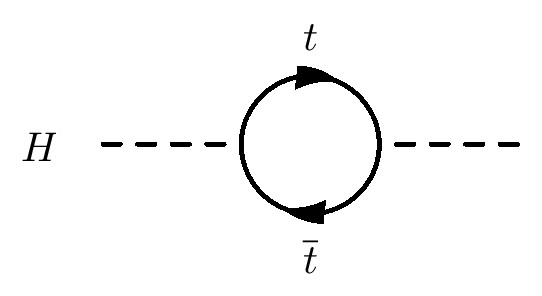
\includegraphics[width= 0.5\linewidth]{images/radiative_corrections_H.png}
    \caption{Leading Feynman diagram for the Higgs radiative corrections; in this case, a quark top and its antiparticle run in the loop. This diagram in particular gives a contribution proportional to the squared value of the considered scale energy}
    \label{radiative_correction}
\end{figure}
To obtain the experimental value, a subtle process of fine-tuning would be needed, so delicate that most of the theorists find it unnatural.\\
A solution would be to consider an intermediate energy scale, around the TeV, that would lead to a more reasonable tuning.
\subsection{Theoretical solutions}
Several solutions have been proposed to solve the known problems of the SM. We report two of the most relevant.\\
\subsubsection{Supersymmetry}
Supersymmetry (SUSY) \cite{susy} is a framework proposed around the 1970s by several physicists independently and that aims to extend the SM.\\
It focuses on the idea that, because of the radiative corrections, the mass of the boson itself should be extremely large. However, this prediction doesn't correspond to the experimental observations made at LHC. \\
SUSY theories predict the existence of several new particles that would help cancel out the contributions to the Higgs mass from the SM particles, allowing the existence of a light Higgs boson. These extra particles are partners of the SM ones, and in particular, would act as a link between the fermions and the bosons, in the sense that a fermionic SM particle would have a bosonic SUSY partner, and vice versa.\\
Because of the internal symmetries of SUSY, the lightest of the newly introduced particles should have a mass of around 100 GeV, and should be stable.\\
However, to date, no relevant experimental indication of the existence of SUSY particles has been observed. \\
LHC, its upgrade HL-LHC and future colliders are expected to further test this framework.\\
\subsubsection{Composite Higgs Models}
Composite Higgs Models (CHM) \cite{chm} consider an alternative approach that assumes the Higgs boson not to be an elementary particle, but a composite state of some new particles. \\
In the models where the Higgs is a Goldstone boson coming from spontaneous symmetry breaking, a larger group of symmetry is considered, which contains the $SU(2)x U(1)$ group of the SM.\\
The larger group then breaks into the SM group that we know, creating a set of (pseudo)Nambu-Goldstone bosons, among which the Higgs boson is included.\\
In CHM, the quadratic divergences from the radiative corrections are solved with the physical cutoff of the compositness scale.\\
To keep a reasonable tuning to the SM, the new energy scale should remain around the TeV scale.\\
LHC, its upgrade HL-LHC and future colliders will be able to test CHM indirectly and directly.

%\section{Why study the self-coupling of the Higgs boson}
\section{Higgs pair production and self-coupling}
In the previous sections, we've discussed the contributions of the Higgs field in the justification of a mass term for the different elementary particles described by the SM.\\
However, we've never explicitly written the complete potential.
And that is because the actual shape of the Higgs potential is unknown.\\
We can rewrite the potential as:
\begin{equation}
    V(\rho(x)) = \frac{1}{2}m_H^2\rho(x)^2 +\lambda v \rho(x)^3 + \frac{1}{4}\lambda\rho(x)^4 +\text{const}
\end{equation}
by expanding the quartic potential and substituting the expansion of the field around the minimum $v$.\\
So, by studying the triple and quartic coupling of the Higgs boson we can study directly the shape of the scalar potential by studying the value of $\lambda$.\\
From the definition of $v$ we can find an explicit form for $\lambda$:
\begin{equation}
    v^2 = -\dfrac{\mu^2}{\lambda} \Longrightarrow \lambda = -\dfrac{\mu^2}{v^2} = \dfrac{m_H^2}{2v^2} 
\end{equation}
Both $m_H$ and $v$ are values observed experimentally, the first by direct measurement, the second by studying the mass of the W and Z bosons, so we have a rough estimate of it:
\begin{equation}
    \lambda \approx 0.13
\end{equation}
The theoretical cross-section for the pair production is, considering only ggF as production mode and with $\sqrt{s}$ = 13 TeV \cite{theoretical_pair_prod}:
\begin{equation}
    \sigma(gg\longrightarrow H H )_{ggF} = 31.31 \text{fb}^{+0.66\%}_{-2.8\%}
\end{equation}
The dominant Feynman diagrams are shown in fig. \ref{pair_prod}. \\
It can be seen that di-Higgs events can be produced via a box diagram, where heavy fermions run (in particular t and b quarks), and via the Higgs boson self-coupling.\\
We can write the interaction Lagrangian as:
\begin{equation}
    - \mathcal{L} =\left(\frac{m_H^2}{2 v} \right)\lambda_{HHH} H^3 + \frac{m_t}{v} \Bar{t}g_t t H,
    \end{equation}
where the first term describes the self-coupling diagram, and the second term describes the box diagram.\\
The two processes interfere destructively, and the cross-section is minimum near the SM value, as can be seen from fig. \ref{cms_coupling}.
This means that a small increase in the value of $\lambda_{HHH}$ decreases the expected HH production cross-section, and so modifies the distributions of event kinematics.
\begin{figure}
    \centering
    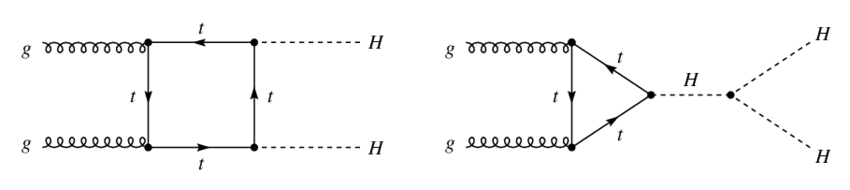
\includegraphics[width= 0.8\linewidth]{images/pair_production.png}
    \caption{Dominant Feynman diagrams for the Higgs pair production. On the left, the box diagram; on the right, the Higgs boson self-coupling-}
    \label{pair_prod}
\end{figure}
    \begin{figure}
    \centering
        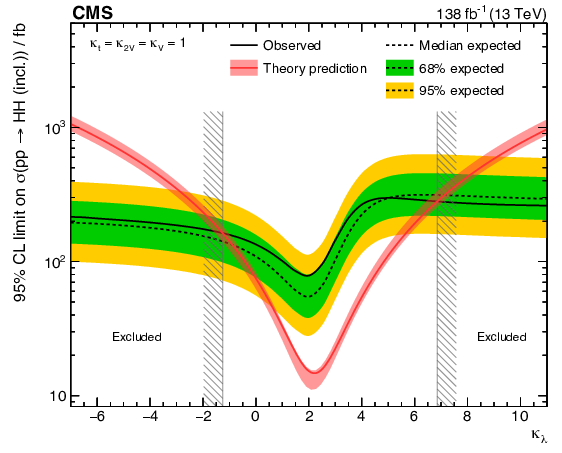
\includegraphics[width=0.8\textwidth]{images/selfcoupling_cms_HH.png}
        \caption{Limits on the Higgs boson self-interaction set from the CMS experiment}
        \label{cms_coupling}    
\end{figure}
To study the self-coupling, the two modes need to be distinguished.\\
It should be noted that because the self-coupling diagram contains a propagator in the s-channel, its relevance should decrease at higher energies because of its behaviour like $1/s$ for energies at the centre of mass considerably higher than $m_H$. Therefore, the box diagram gives on average more energetic Higgs boson pairs than the triangle diagram, so the opening angle between the decay products of each boson can be useful to isolate the self-coupling diagram \cite{theo_pair}.\\
There is also an alternative approach to studying the self-coupling of the Higgs boson, and that is to measure deviations of the inclusive and differential single H production rates \cite{HL-LHC_Higgs}. The contributions of the self-coupling in the single H production can be mainly found in the production in association with top quarks ($t\Bar{t}H$) or single-top production (tH), because of the large mass of the top quark, and consequently, the large coupling with the Higgs boson.\\
A study of the differential production cross-section as a function of the distribution of $p_T^H$ can be done, for example, considering $\gamma\gamma$ as a final state for the possibility of having a fully reconstructed event, and from which the effects of a modified H boson self-coupling can be extrapolated.\\
This gives an ulterior mode to test the physics of the SM Higgs boson, complementary to the direct search of Higgs pair production.
%\subsection{Possible implications of the HH measurements}
%A brief summary of possible results closely related to the Higgs pair production are listed.
%\subsubsection{Electroweak phase transition}
%One of the open problems of high energy physics and cosmology is the origin of matter-antimatter asymmetry. One of the solutions proposed is the electroweak baryogenesis, where the asymmetry is tied to the electroweak symmetry breaking. In this scenario, the universe is supposed to have gone from electroweak symmetric to broken phase at a temperature T$_{EW} \sim 100$ GeV. If such a transition occurred, there must have been some CP-violating interactions that were active in those instants and that justify the now observed asymmetry. However, the current formulation of the SM doesn't meet any of these two requirements: the symmetry breaking given from a 125 GeV Higgs boson doesn't cause the phase transition, and the CP violation from the $V_{CKM}$ isn't enough to justify the observed asymmetry. For this reason, viable electroweak baryogenesis needs BSM physics that couples with the Higgs boson.\\
%Deviation from the SM pair production cross-section and anomalous self-coupling can be a viable way to indirectly probe the existence of new interactions needed for the electroweak phase transition to occur even with a 125 GeV Higgs boson.
%\subsubsection{Vacuum stability}

\subsection{Results on the measurement}
\subsubsection{CMS}
The following results were published in 2022. In plot \ref{cms_results} we show the ratio between the observed cross-section and the SM one for Higgs pair production, divided per year and per final state (and their combination). \\
\begin{figure}[ht]
    \centering
        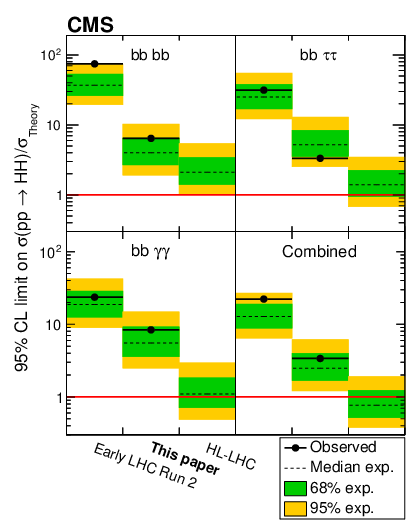
\includegraphics[width=0.7\textwidth]{images/cms_expected_HH_time.png}
        \caption{Recent results and projections from the CMS experiment on the production of Higgs pairs}
    \label{cms_results}  
\end{figure}
A 95\% confidence level observed (expected) upper limit on the combined non-resonant production cross-section is set at \cite{res_CMS_combined}:
\begin{equation}
    \sigma_{obs} \left(\sigma_{exp}\right) = 3.4 (2.5)\text{  }\sigma_{SM}
\end{equation}
\subsubsection{ATLAS}
The following results were published in 2023\cite{atlas_combined}. In plot \ref{atlas_results} we show the cross-section measured in the various decay channels (and their combination)\\
A 95\% confidence level observed (expected) upper limit on the combined non-resonant production cross-section is set at:
\begin{equation}
        \sigma_{obs} \left(\sigma_{exp}\right) = 2.4 (2.9)\text{  }\sigma_{SM}
\end{equation}
on the double-Higgs signal strength, defined as the sum of the ggF HH and VBF HH production cross-sections normalised to its SM prediction
\begin{figure}[ht]
    \centering
        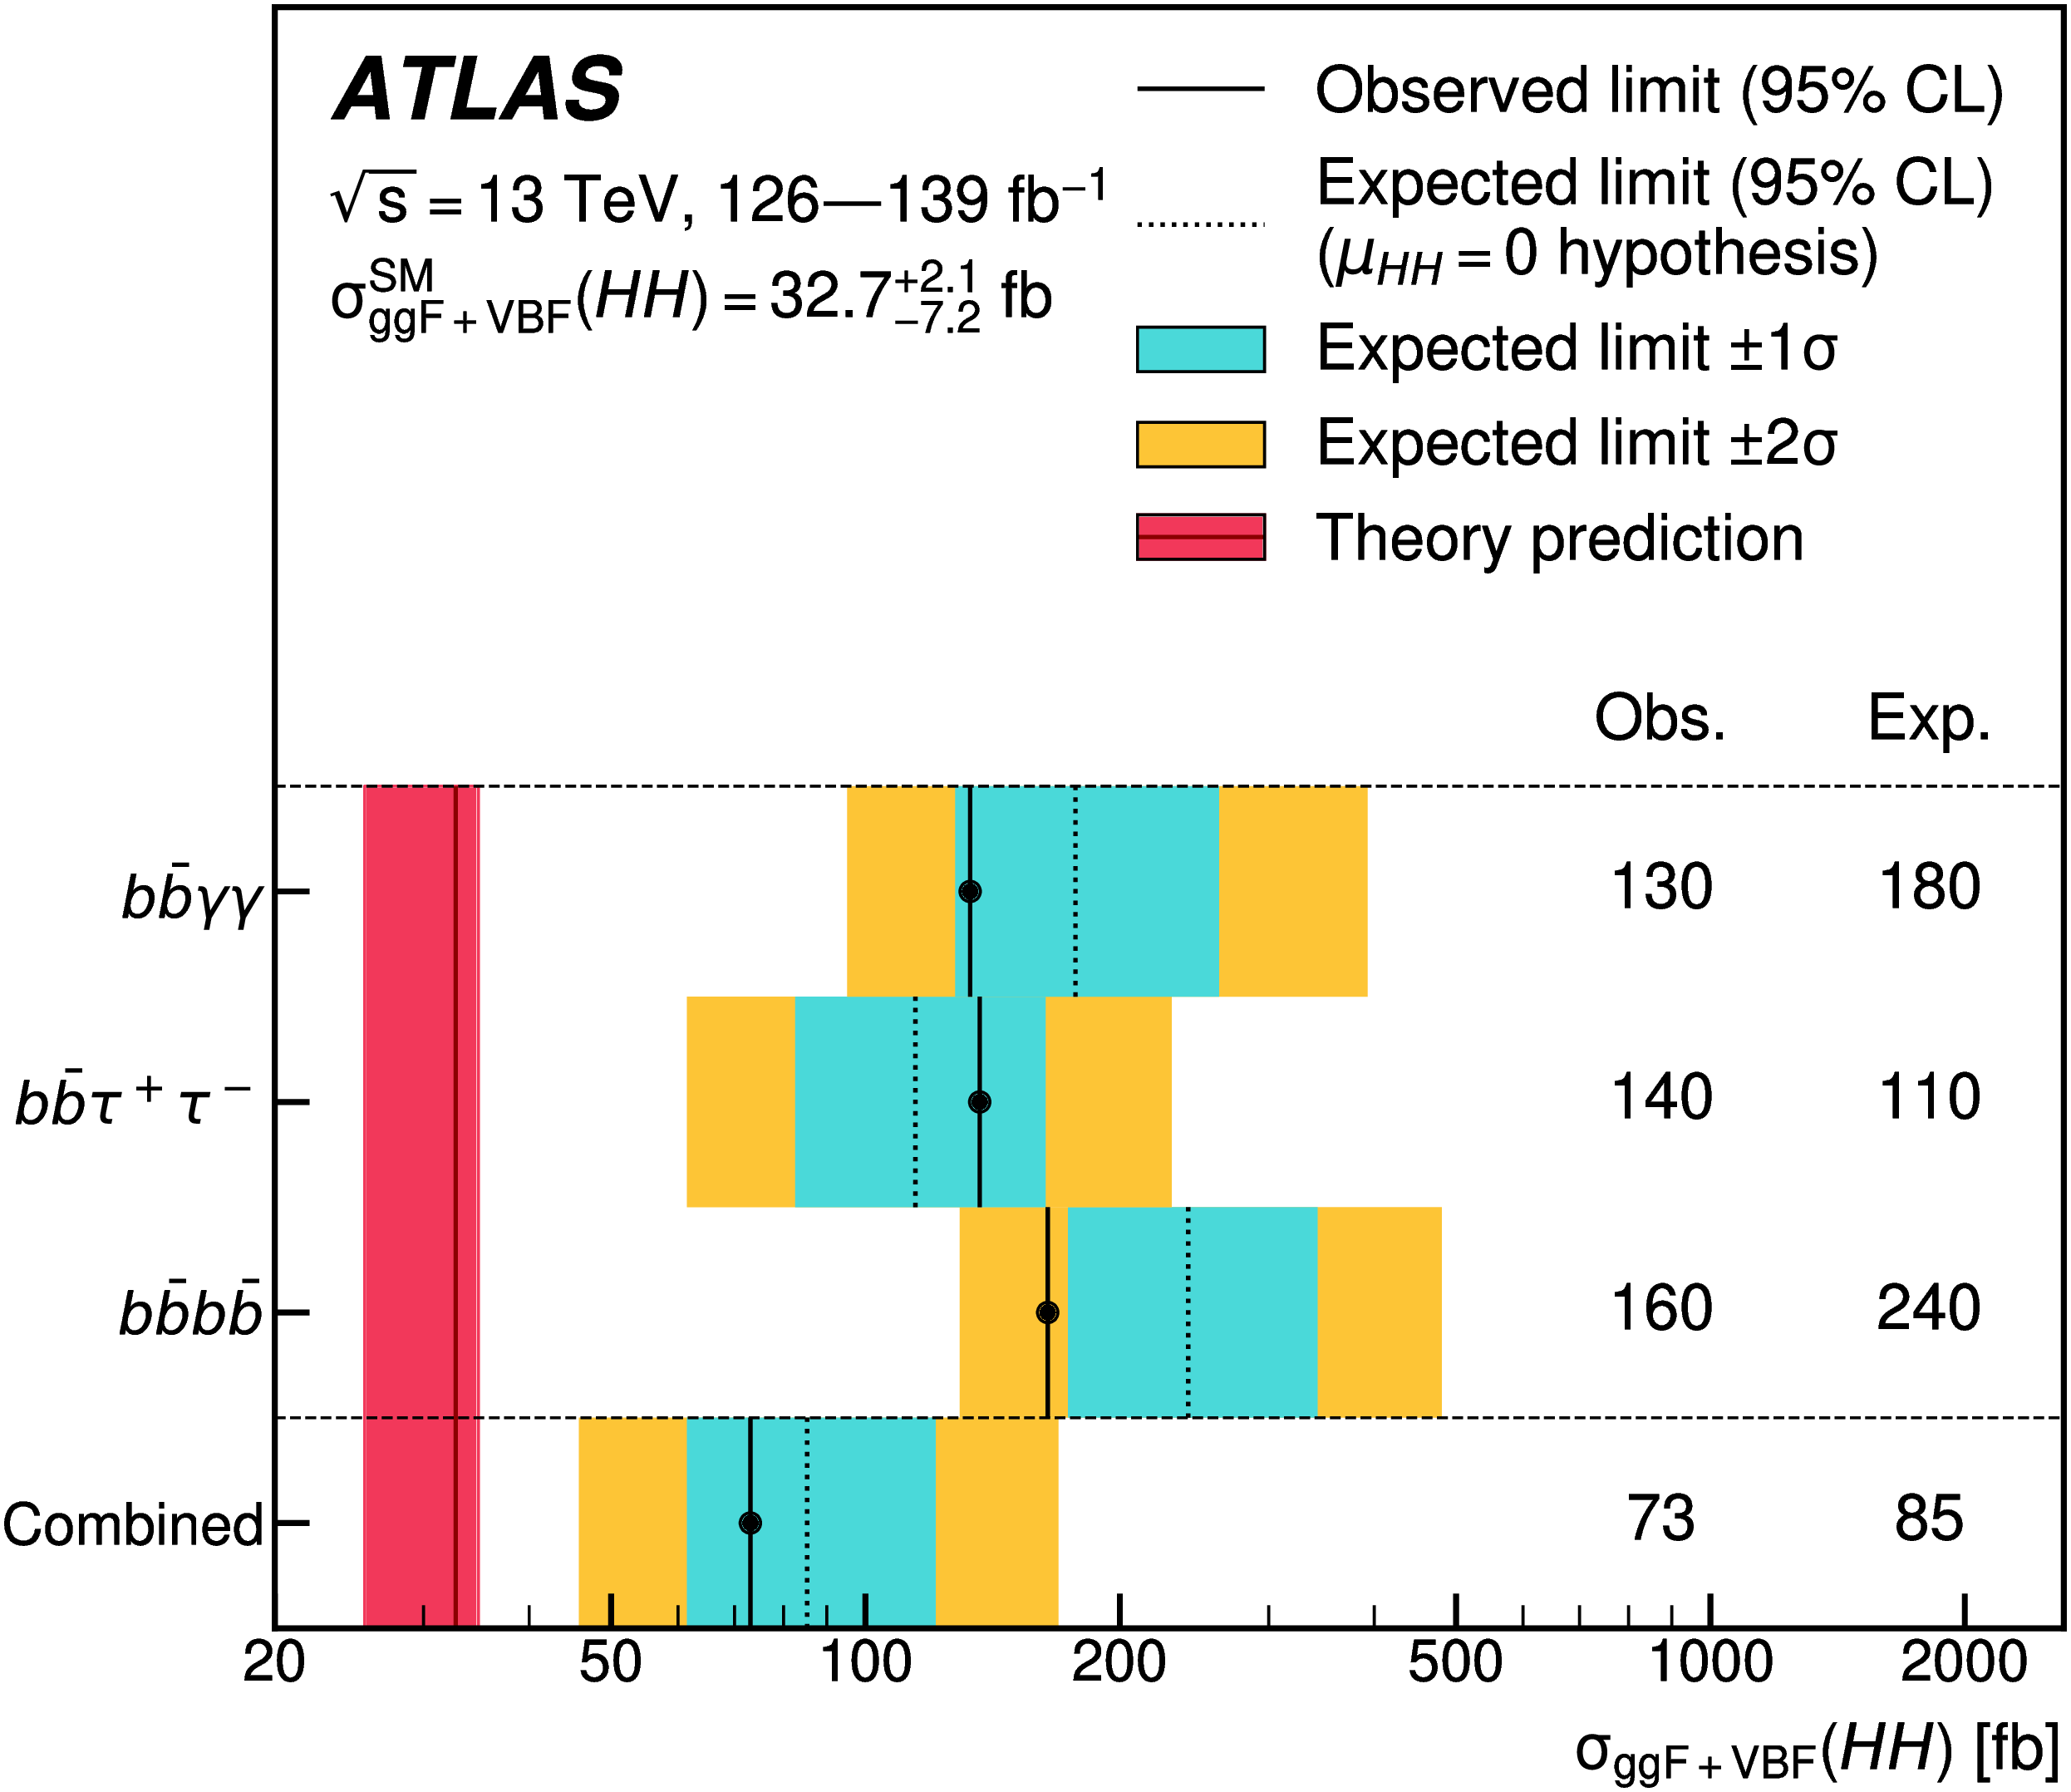
\includegraphics[width=0.7\textwidth]{images/atlas_expected.png}   
    \caption{Limits on the production of Higgs boson pairs set by the experiment ATLAS}
    \label{atlas_results}  
\end{figure}